% https://en.wikipedia.org/wiki/Cut_(graph_theory)
\section{Puentes}\label{bridges}
Una arista se llama puente si al eliminarla del grafo (manteniendo los vértices) aumenta el número de componentes conectados.

\begin{figure}[H]
	\centering
	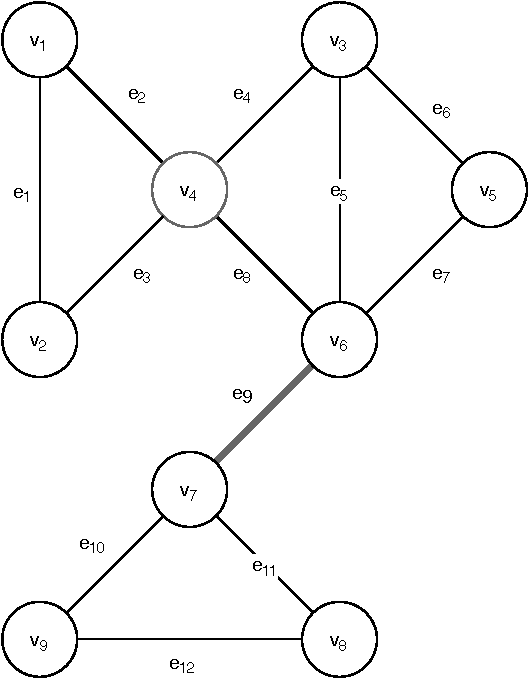
\includegraphics[width=0.4\linewidth]{document/ArticulationPoints/images/example-of-bridge}
	\caption{Ejemplo de grafo con una arista puente \( e_9 \).}
	\label{fig:connected-disconnected-graph}
\end{figure}
